\documentclass[12pt]{article}
\pagestyle{empty}
\usepackage{amsmath, amssymb, amsthm}
\usepackage{latexsym, epsfig, ulem, cancel, multicol, hyperref}
\usepackage{graphicx, tikz, subfigure,pgfplots}
\usepackage[margin=1in]{geometry}
\setlength{\parindent}{0pt}
\usepackage{multirow}
\usepackage{mathtools}
\usepackage{color}


\usepackage{verbatim}
\usepackage{tikz}
\usepackage{pgfplots}

\newcommand{\T}[0]{\top}
\newcommand{\F}[0]{\bot}
\newcommand{\liminfty}[1]{\lim_{#1 \to \infty}}
\newcommand{\limzero}[1]{\lim_{#1 \to 0}}
\newcommand{\Z}{\mathbb{Z}}
\newcommand{\R}{\mathbb{R}}
\newcommand{\C}{\mathbb{C}}
\newcommand{\Q}{\mathbb{Q}}
\newcommand{\lineint}[1]{\int_{#1}}
\newcommand{\pypx}[2]{\frac{\partial #1}{\partial #2}}
\newcommand{\divg}{\nabla \cdot}
\newcommand{\curl}{\nabla \times}
\newcommand{\dydx}[2]{\frac{d #1}{d #2}}
\newcommand{\sqbkt}[1]{\left[ #1 \right]}
\newcommand{\paren}[1]{\left( #1 \right)}
\newcommand{\tribkt}[1]{\left< #1 \right>}
\newcommand{\abso}[1]{\left|#1 \right|}

\newcommand{\defcomp}{\exists r,s\in \Z^+ \paren{n=rs \wedge \paren{1<r<n} \wedge \paren{1<s<n}}}
\newcommand{\defprime}{\forall r,s \in \Z ^+ \paren{n=rs \rightarrow \paren{r = 1 \wedge s = n}\veebar \paren{r=n \wedge s=1}}}

\newcommand{\redt}{\textcolor{red}{T}}
\newcommand{\redf}{\textcolor{red}{F}}

\newcommand{\wsnumber}{1}
\newcommand{\wstopic}{Vectors}
\pgfplotsset{
    every linear axis/.append style={
       axis x line=center,
       axis y line=center,
       xlabel={$x$},
       ylabel={$y$}
    },
    every axis plot/.append style={thick,mark=none}
}
\tikzset{
    point/.style={circle,draw,fill,minimum width=0.3ex,inner sep=0pt,outer sep=0pt},
    every label/.append style={black}
}


\usepackage[margin=1in]{geometry}
\usepackage{amsmath, amssymb, amsthm, graphicx, hyperref}
\usepackage{enumerate}
\usepackage{fancyhdr}
\usepackage{multirow, multicol}
\usepackage{tikz}
\pagestyle{fancy}
\fancyhead[RO]{Dennis Li}
\fancyhead[LO]{Summer 6W2 2024 MA-UY 2314}
\usepackage{comment}
\newif\ifshow
\showfalse

\ifshow
  \newenvironment{solution}{\textbf{Solution.}}{}
\else
  \excludecomment{solution}
\fi

\renewcommand{\thefootnote}{\fnsymbol{footnote}}
\usepackage{comment}


\newtheorem*{remark}{Remark}


\begin{document}

    \begin{center}
    \ifshow
      \textbf{\Large Homework 2 Solution}\\
    \else
      \textbf{\Large Homework 2}\\
    \fi
    Due: Tuesday July 16\\via Gradescope\\
    \end{center}
    
    \hrule
    
    \vspace{0.2cm}
    
    \begin{enumerate}[$\bullet$]  
    \item Late homework is not accepted.  Lateness due to technical issues will not be excused.  
    \end{enumerate}
    
    \hrule
    
    \vspace{0.5cm}
    
    
    
    \begin{enumerate}
    
        \item Section 2.3 \#9, 12(b), 23
            \begin{enumerate}
                \item[9.]
                    \begin{align*}
                        & p \wedge q \rightarrow \neg r \\
                        & p \vee \neg q\\
                        & \neg q \rightarrow p\\
                        & \therefore \neg r
                    \end{align*}
                    \[
                        \begin{tabular}{|c|c|c|c|c|c|c|c|c|c|}
                        \hline
                        $p$ & $q$ & $r$ & $p \wedge q$ & $\neg r$ & $p \wedge q \rightarrow \neg r$ & $\neg q$ & $p \vee \neg q$ & $\neg q \rightarrow p$ & $\neg r$ \\
                        \hline
                        T & T & T & T & F & F & F & T & T & F \\
                        \hline
                        T & T & F & T & T & \redt & F & \redt & \redt & \redt \\
                        \hline
                        T & F & T & F & F & T & T & T & T & F \\
                        \hline
                        T & F & F & F & T & \redt & T & \redt & \redt & \redt \\
                        \hline
                        F & T & T & F & F & T & F & F & F & F \\
                        \hline
                        F & T & F & F & T & T & F & F & F & T \\
                        \hline
                        F & F & T & F & F & \redt & T & \redt & \redt & \redf \\
                        \hline
                        F & F & F & F & T & \redt & T & \redt & \redt & \redt \\
                        \hline
                        \end{tabular}
                    \]
                Observing the highlighted critical row, it can be identified that all premises are true on the 7th row, yet the conclusion is false. While on the other highlighted row, all premises are true therefore the conclusion is true. This indicates that the argument is invalid. 


                \item[12(b).]
                    \begin{align*}
                        & p \rightarrow q\\
                        & \neg p\\
                        & \therefore \neg q
                    \end{align*}
                    \[
                    \begin{tabular}{|c|c|c|c|c|}
                        \hline
                        $p$ & $q$ & $p \rightarrow q$ & $\neg p$ & $\neg q$ \\
                        \hline
                        T & T & T & F & F \\
                        \hline
                        T & F & F & F & T \\
                        \hline
                        F & T & \redt & \redt & \redf \\
                        \hline
                        F & F & \redt & \redt & \redt \\
                        \hline
                    \end{tabular}
                    \]

                All premises are true on the 3rd row, however the conclusion is false, therefore this is an invalid argument. 

                \item[23.] We first define the following:
                \[
                p:= \text{ Oleg is a math major}
                \]
                \[
                q:= \text{ Oleg is an economics major}
                \]
                \[
                r:= \text{ Oleg is required to take Math 362}
                \]
                The argument is
                \begin{align*}
                    & p \vee q\\
                    & p \rightarrow r\\
                    \therefore & q \rightarrow \neg r
                \end{align*}

                \[
                \begin{tabular}{|c|c|c|c|c|c|c|}
                    \hline
                    $p$ & $q$ & $r$ & $p \vee q$ & $p \rightarrow r$ & $q \rightarrow \neg r$ \\
                    \hline
                    T & T & T & \redt & \redt & \redf \\
                    \hline
                    T & T & F & T & F & T \\
                    \hline
                    T & F & T & \redt & \redt & \redt \\
                    \hline
                    T & F & F & T & F & T \\
                    \hline
                    F & T & T & \redt & \redt & \redf \\
                    \hline
                    F & T & F & \redt & \redt & \redt \\
                    \hline
                    F & F & T & F & T & T \\
                    \hline
                    F & F & F & F & T & T \\
                    \hline
                    \end{tabular}
                \]
                By looking at the 1st row and the 5th row, all premises are true yet the conclusion is false. Therefore this is an invalid argument. 
            \end{enumerate}
            \newpage

        \item Section 2.3 \#29,38(d)
            \begin{enumerate}
                \item[29] If at least one of these two numbers is divisible by 6, then the product of these two numbers is divisible by 6. \\
                Neither of these two numbers is divisible by 6.\\
                Therefore the product of these two numbers is not divisible by 6.\\
                \\
                Let $a,b$ be two numbers. 
                \begin{align*}
                    & 6 \mid a \vee 6 \mid b \rightarrow 6 \mid ab\\
                    & 6 \nmid a \wedge 6 \nmid b\\
                    \therefore & 6 \nmid ab
                \end{align*} 
                The contrapositive of the original statement should be
                \[
                6 \nmid ab \rightarrow 6 \nmid a \wedge 6 \nmid b
                \]
                However the argument suggests that
                \[
                6 \nmid a \wedge 6 \nmid b \rightarrow 6 \nmid ab 
                \]
                Therefore it is an inverse error. 

                \item[38(d).] Assume U is knight, then U,V,W,X,Y,Z are all knaves. This implies that U is speaking truth and is a knight, which contradicts with U, therefore U is a knave.\\
                Then assume V and W are both true, that implies there are exactly 3 knights. This means that X,Y,Z are all knaves, but U is also a knave which contradicts with the assumption, therefore either V is a knave or W is a knave.\\
                Now assume V is a knight, and W is a knave, then U,W,Y,Z are all knaves, which contradicts with the assumption, therefore V has to be a knave. \\
                Consider W to be a knight, then U,V,X are all knaves, either Y or Z is a knight, we examine individual cases.\\
                If W and Z are knights, that means there are only one knight, and W would be true, which contradicts with the assumption that Z is a knight. Therefore Z is a knave.\\
                If W and Y are knights, U,V,X,Z are knaves, which has no logical contradictions.\\
                Therefore W and Y are knights. 
            \end{enumerate}
        \newpage

            
        \item Section 2.3 \# 42, 44. Annotate.
            \begin{enumerate}
                \item[42.]
                    \begin{align*}
                                    & q \rightarrow r \\
                                    & \neg r\\
                        \therefore \;  & \neg q                        & \text{Modus Tollens}\\
                                    &\neg q \rightarrow u \wedge s \\
                        \therefore \;  & u \wedge s                    & \text{Modus Ponens}\\
                                    & u \wedge s\\
                        \therefore  \; & s                             & \text{Specialization}\\
                                    & p \vee q\\
                                    & \neg q\\
                        \therefore \; & p                             & \text{Elimination}\\
                                    & p\\
                                    & s\\
                        \therefore  & p\wedge s                       & \text{Conjunction}\\
                                    & p \wedge s \rightarrow t\\
                        \therefore \; & t                             & \text{Modus Ponens}
                    \end{align*}
                \item[44.]
                    \begin{align*}
                                    & \neg q \vee s\\
                                    & \neg s\\
                        \therefore  & \neg q                          & \text{Elimination}\\
                                    & p \rightarrow q\\
                                    & \neg q\\
                        \therefore  & \neg p                          & \text{Modus Tollens}\\
                                    & \neg s \rightarrow \neg t\\
                                    & \neg s\\
                        \therefore  & \neg t                          & \text{Modus Ponens}\\
                                    & r \vee s\\
                                    & \neg s\\
                        \therefore  & r                               & \text{Elimination}\\
                                    & \neg p\\
                        \therefore  & \neg p \wedge r                 & \text{Conjunction}\\
                                    & \neg p \wedge r \rightarrow u\\
                        \therefore  & u                               & \text{Modus Ponens}\\
                                    & w \vee t\\
                                    & \neg t\\
                        \therefore  & w                               & \text{Elimination}\\
                                    & u\\
                        \therefore  & u \wedge w                      & \text{Conjunction}
                    \end{align*}
            \end{enumerate}
        \newpage
        \item Section 3.1 \# 4, 20, 32(b)(d).
            \begin{enumerate}
                \item[4.] Let $Q(x,y)$ be the predicate \textit{If $x<y$ then $x^2 < y^2$} with the domain $\forall x,y \in \R$
                    \begin{enumerate}[a.]
                        \item Explain why $Q(x,y)$ is false if $x=-2$ and $y=1$
                            \[
                            Q(-2,1) \equiv \paren{-2}^2 < 1^2
                            \]
                            \[
                            \equiv 4 < 1
                            \]
                            Which is a false statement, therefore the predicate is false with the given input. 
                        \item Give values different from those in (a.) which makes $Q(x,y)$ false.
                            \[
                            \text{let $x=-3$ and $y=2$}
                            \]
                            \[
                            Q(-3,1) \equiv \paren{-3}^2 < 2^2 \equiv 9 < 4
                            \]
                            Which is a false statement, therefore the predicate is false with the given input. 
                        \item Explain why $Q$ is true if $x=3 \;\;\; y=8$
                            \[
                            Q(3,8) \equiv 3^2 < 8^2 \equiv 9 < 64
                            \]
                            Which is a true statement, therefore the predicate is true with the given input.
                        \item Give values different from those in (a.) which makes $Q(x,y)$ true. 
                            \[
                            \text{let $x=2$ and $y=3$}
                            \]
                            \[
                            Q(2,3) \equiv 2^2 < 3^2 \equiv 4 < 9
                            \]
                            Which is a true statement, therefore the predicate is true with the given input.
                    \end{enumerate}
                \item[20.]Rewrite the following statement informally in at least two different ways without using variables or qualifiers.
                \[
                \text{If a real number is positive, then it's square root is positive. }
                \]
                \[
                \text{The square root of any positive real number is positive.}
                \]
                \item[32(b)(d).] Let $\R$ be the domain of the predicate variable $x$. Which of the following are true and which are false, give counter examples for the statements that are false. 
                    \begin{enumerate}
                        \item[b.] $x>2 \Rightarrow x^2 > 4$\\
                        This statement is true.
                        \item[d.] $x^2 > 4 \iff \abso{x} >2$\\
                        This statement is true.
                        
                    \end{enumerate}
                    
                
            \end{enumerate}
        \newpage
        \item Section 3.2 \#15 (b)(d)(e).
            \begin{enumerate}
                \item[b.]Let \( D = \{-48, -14, -8, 0, 1, 3, 16, 23, 26, 32, 36\} \). Determine which of the following statements are true and which are false. Provide counterexamples for the statements that are false.

                    \begin{enumerate}
                        \item[b.] \(\forall x \in D\), if \( x \) is less than 0 then \( x \) is even.\\
                        The statement is true.
                        \item[d.] \(\forall x \in D\), if the ones digit of \( x \) is 2, then the tens digit is 3 or 4.\\
                        The statement is true.
                        \item[d.] \(\forall x \in D\), if the ones digit of \( x \) is 6, then the tens digit is 1 or 2.\\
                        The statement is false for $x=36$.
                    \end{enumerate}
            \end{enumerate}
        \newpage
        \item Section 3.2 \#12, 40, 46.
            \begin{enumerate}
                \item[12.] Statement: The product of any irrational number and any rational number is irrational.\\
                        Proposed Negation: The product of any irrational number and any rational number is rational.\\
                        The correct negation is\\  
                        There exists an irrational number and a rational number such that their product is rational.\\

                \item[40.]Being divisible by 8 is sufficient condition for being divisible by 4.\\
                If a number is divisible by 8, then the number is divisible by 4. 

                \item[46.]Having a large income is not a necessary condition for a person to be happy\\
                A person can have a large income and not be happy.
                    
                
                      
            \end{enumerate}

            
        \newpage
        \item Section 3.3 \#43, 44, 45
            \begin{enumerate}
                \item[43.]The following is the definition for \(\lim_{x \to a} f(x) = L\): For every real number \(\epsilon > 0\), there exists a real number \(\delta > 0\) such that for every real number \(x\), if \(a - \delta < x < a + \delta\) and \(x \neq a\) then
                \[
                L - \epsilon < f(x) < L + \epsilon.
                \]
                Write what it means for \(\lim_{x \to a} f(x) \neq L\). In other words, write the negation of the definition.\\
                The negation means that,  there exists a real number $\epsilon > 0$, such that for every real number $\delta >0$ there exists a real number $x$ such that,  $a-\delta < x < a + \delta $ and $x \neq a$ and
                \[
                L- \epsilon \geq f(x) \vee f(x) \geq L+\epsilon 
                \]

                \item[44.] Explain if the follow is true of false:
                    \begin{enumerate}[a.]
                        \item $\exists ! x \in \R \; \forall y \in \R \paren{xy=y}$\\
                        This is a true statement. The unique real number is $x=1$, which is the \textit{multiplicative identity}.
                        \item $\exists ! x \in \Z \paren{ \frac{1}{x} \in \Z}$\\
                        This is a true statement. The unique real number is $x=1$, which satisfy the argument since 
                        \[
                        \frac{1}{1} = 1 \in \Z
                        \]
                        \item $\forall x \in \R \; \exists ! y \in \R \paren{x+y=0}$\\
                        This is a true statement. 
                        \begin{align*}
                            \text{Let $x \in \R$, choose $y=-x\in \R$}\\
                            x+y = x + (-x) = 0
                        \end{align*}
                    \end{enumerate}
                \item[45.] Suppose P(x) is a predicate and D is the domain of $x$, rewrite the statement \[
                \exists ! x \in D \paren{P(x)}\]
                Rewrite:
                There exists a unique $x$ in domain $D$ such that $P(x)$ is true.
               
                
            \end{enumerate}
                
        \newpage
        \item Section 3.3 \#56, 57.
            \begin{enumerate}
                \item[56.] \(\exists x \in D :\; (P(x) \wedge Q(x)), \text{ and } (\exists x \in D: P(x)) \wedge (\exists x \in D: Q(x))\)\\
                if $D$ contains some values of $x$ that satisfies $P(x)$ and some other values that satisfy $Q(x)$ but does not satisfy $P(x)$, then the first part would be false, but the second part would be true.
                \item[57.] \(\forall x \in D: \; (P(x) \vee Q(x)), \text{ and } (\forall x \in D: P(x)) \vee (\forall x \in D: Q(x))\)\\
                if $D$ contains some values of $x$ that satisfies $P(x)$ and some other values that satisfy $Q(x)$ but does not satisfy $P(x)$, the first half would be true, but the second half would be false. 
            \end{enumerate}



        \newpage
        \item Section 3.4 \#30
            \begin{enumerate}[$a:$]
                \item 	$\forall$ objects $x$, If an object $x$ is above all the triangles, then $x$ is above all the blue objects. $\forall$ objects $x$, 
                \item   $\forall$ objects $x$,  If an object $x$ is not above all the gray objects, then $x$ is not a square.\\
                Contrapositive $b'$: If an object $x$ $\forall$ objects $x$, is a square, then $x$ is above all gray objects.
                \item   $\forall$ objects $x$,  If an object $x$ is black, then it is a square.
                \item 	$\forall$ objects $x$,  If an object $x$ is above all the gray objects, then $x$ is above all the triangles.
                \item[$\therefore$] $\forall$ objects $x$,  If an object $x$ is black, then $x$ is above all the blue objects.
            \end{enumerate}
            Re-arrange the above statements
            \begin{enumerate}
                \item[$c:$]  $\forall$ objects $x$,  If an object $x$ is black, then it is a square.
                \item[$b':$] $\forall$ objects $x$,  If an object $x$ is a square, then $x$ is above all gray objects.
                \item[$d:$]  $\forall$ objects $x$,  If an object $x$ is above all the gray objects, then $x$ is above all the triangles.
                \item[$a:$]  $\forall$ objects $x$,  If an object $x$ is above all the triangles, then $x$ is above all the blue objects.
                \item[$\therefore$]  $\forall$ objects $x$,  If an object $x$ is black, then $x$ is above all the blue objects.
            \end{enumerate}
            Here are sketch of the statements.
            \begin{enumerate}[i.]
                \item 
                        \begin{figure}[!h]
                            \centering
                            \includegraphics[width=0.25\linewidth]{Picture Folder//HW02/3.4-30-c.png}
                            \caption{statement $c$}
                            \label{fig:3.4-30-c}
                        \end{figure}
                \newpage
                \item 
                        \begin{figure}[!h]
                            \centering
                            \includegraphics[width=0.25\linewidth]{Picture Folder//HW02/3.4-30.b'.png}
                            \caption{statement $b'$}
                            \label{fig:3.4-30-b'}
                        \end{figure}

                \item 
                        \begin{figure}[!h]
                            \centering
                            \includegraphics[width=0.25\linewidth]{Picture Folder//HW02/3.4-30-d.png}
                            \caption{statement $d$}
                            \label{fig:3.4-30-d}
                        \end{figure}

                \item
                        \begin{figure}[!h]
                            \centering
                            \includegraphics[width=0.25\linewidth]{Picture Folder//HW02/3.4-30-a.png}
                            \caption{Statement $a$}
                            \label{fig:3.4-30-a}
                        \end{figure}
                \newpage
                \item
                        \begin{figure}[!h]
                            \centering
                            \includegraphics[width=0.25\linewidth]{Picture Folder//HW02/3.4-30-con.png}
                            \caption{Conclusion}
                            \label{fig:3.4-30-con}
                        \end{figure}
            
            
            \end{enumerate}
        
            
        \newpage


        \item Section 3.4 \#32, 34.

            \begin{enumerate}
                \item[32.]
                    \begin{enumerate}
                        \item $\forall$ example $x$, if there is an $x$, then $x$ is not arranged in regular order.
                        \item $\forall$ example $x$, If the examples are not arranged in regular order like the ones I am used to, then I do not understand $x$.
                        \item $\forall$ example $x$, If I do not understand $x$, then I grumble.
                        \item $\forall$ example $x$, If I grumble, then $x$ give me a headache.
                        \item $\forall$ example $x$, If $x$ give me a headache, then $x$ are not easy.
                        \item[$\therefore$] $\forall$ example $x$, these $x$ are not easy.
                    \end{enumerate}
                    \begin{enumerate}
                        \item If I do not grumble while working a logic example, then I understand it.
                        \begin{center}
                        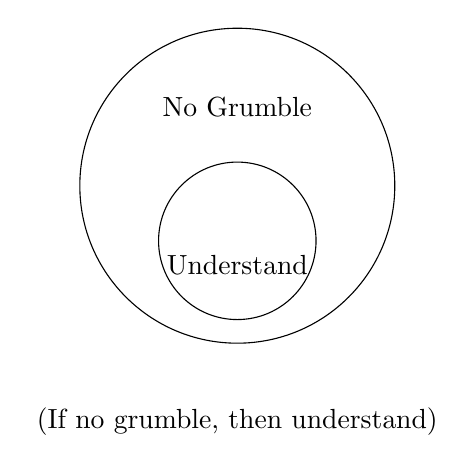
\begin{tikzpicture}
                            \draw (0,0) circle (2cm);
                            \draw (0,-0.7) circle (1cm);
                            \node at (0,-1) {Understand};
                            \node at (0,1) {No Grumble};
                            \node at (0,-3) {(If no grumble, then understand)};
                        \end{tikzpicture}
                        \end{center}
                        
                        \item The arguments in these examples are not arranged in regular order like the ones I am used to.
                        \begin{center}
                        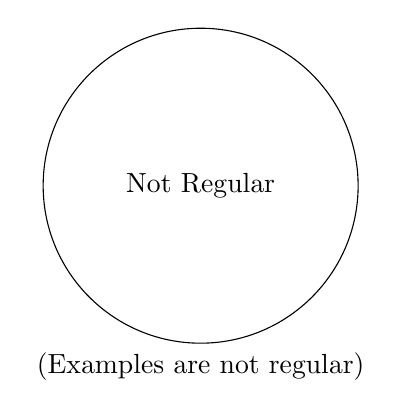
\begin{tikzpicture}
                            \draw (0,0) circle (2cm);
                            \node at (0,0) {Not Regular};
                            \node at (0,-2.3) {(Examples are not regular)};
                        \end{tikzpicture}
                        \end{center}
                        
                        \item If an example is easy, then it does not make my head ache.
                        \begin{center}
                        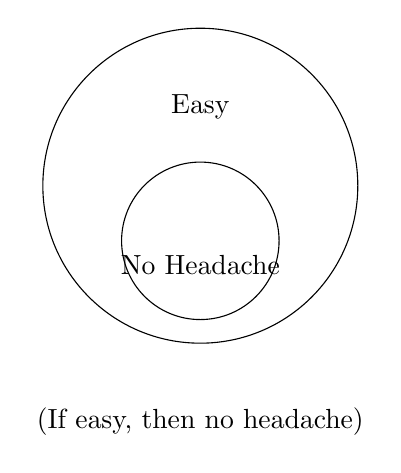
\begin{tikzpicture}
                            \draw (0,0) circle (2cm);
                            \draw (0,-0.7) circle (1cm);
                            \node at (0,-1) {No Headache};
                            \node at (0,1) {Easy};
                            \node at (0,-3) {(If easy, then no headache)};
                        \end{tikzpicture}
                        \end{center}
                        
                        \item If the arguments are not arranged in regular order like the ones I am used to, then I do not understand the examples.
                        \begin{center}
                        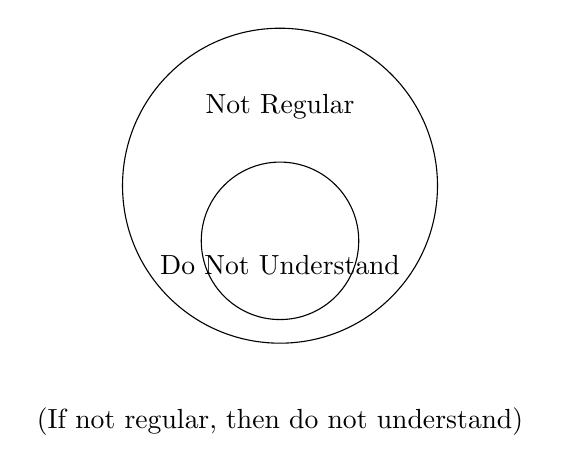
\begin{tikzpicture}
                            \draw (0,0) circle (2cm);
                            \draw (0,-0.7) circle (1cm);
                            \node at (0,-1) {Do Not Understand};
                            \node at (0,1) {Not Regular};
                            \node at (0,-3) {(If not regular, then do not understand)};
                        \end{tikzpicture}
                        \end{center}
                        
                        \item If an example does not give me a headache, then I do not grumble at it.
                        \begin{center}
                        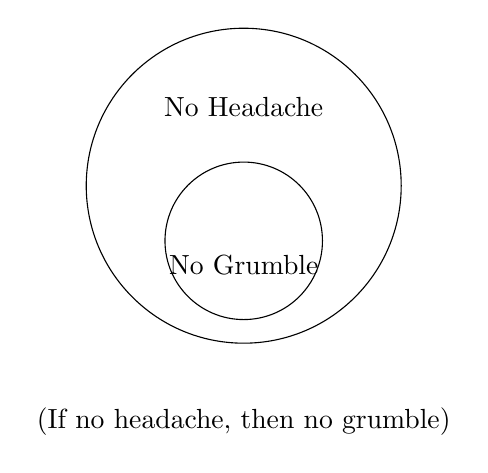
\begin{tikzpicture}
                            \draw (0,0) circle (2cm);
                            \draw (0,-0.7) circle (1cm);
                            \node at (0,-1) {No Grumble};
                            \node at (0,1) {No Headache};
                            \node at (0,-3) {(If no headache, then no grumble)};
                        \end{tikzpicture}
                        \end{center}
                    \end{enumerate}

                \item[34.]
                    \begin{enumerate}
                        \item $\forall$ writer $x$, If $x$ is Shakespeare, then $x$ wrote Hamlet.
                        \item $\forall$ writer $x$, If $x$ wrote Hamlet, then $x$ is a true poet.
                        \item $\forall$ writer $x$, If $x$ is a true poet, then they can stir the human heart.
                        \item $\forall$ writer $x$, If $x$ can stir the human heart, then $x$ understand human nature.
                        \item $\forall$ writer $x$, If $x$ understands human nature, then $x$ are clever.
                        \item[$\therefore$] $\forall$ writer $x$, If $x$ is Shakespeare, then $x$ is clever.

                    \end{enumerate}
                    \begin{enumerate}
                        \item For all writers \( x \), if \( x \) is Shakespeare, then \( x \) wrote Hamlet.
                        \begin{center}
                        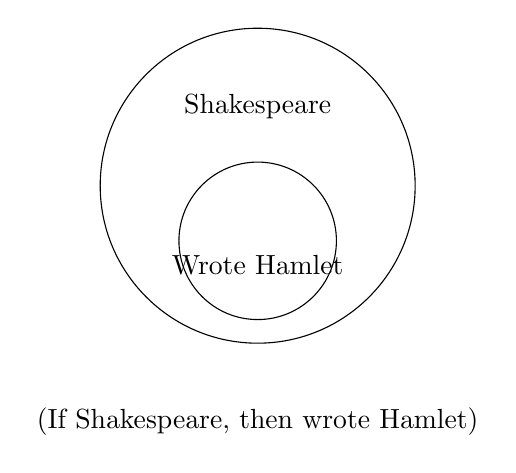
\begin{tikzpicture}
                            \draw (0,0) circle (2cm);
                            \draw (0,-0.7) circle (1cm);
                            \node at (0,-1) {Wrote Hamlet};
                            \node at (0,1) {Shakespeare};
                            \node at (0,-3) {(If Shakespeare, then wrote Hamlet)};
                        \end{tikzpicture}
                        \end{center}
                        
                        \item For all writers \( x \), if \( x \) wrote Hamlet, then \( x \) is a true poet.
                        \begin{center}
                        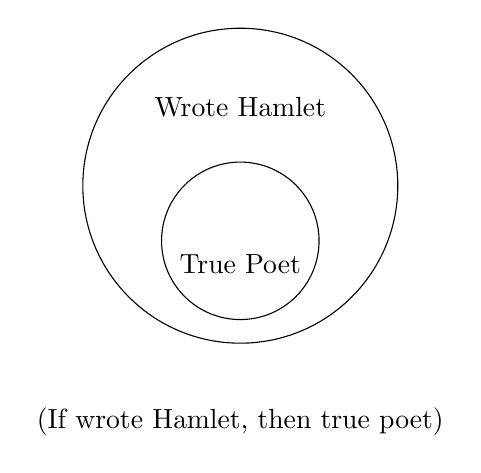
\begin{tikzpicture}
                            \draw (0,0) circle (2cm);
                            \draw (0,-0.7) circle (1cm);
                            \node at (0,-1) {True Poet};
                            \node at (0,1) {Wrote Hamlet};
                            \node at (0,-3) {(If wrote Hamlet, then true poet)};
                        \end{tikzpicture}
                        \end{center}
                        
                        \item For all writers \( x \), if \( x \) is a true poet, then they can stir the human heart.
                        \begin{center}
                        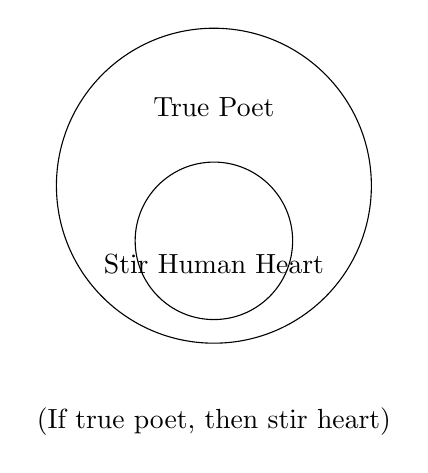
\begin{tikzpicture}
                            \draw (0,0) circle (2cm);
                            \draw (0,-0.7) circle (1cm);
                            \node at (0,-1) {Stir Human Heart};
                            \node at (0,1) {True Poet};
                            \node at (0,-3) {(If true poet, then stir heart)};
                        \end{tikzpicture}
                        \end{center}
                        
                        \item For all writers \( x \), if \( x \) can stir the human heart, then \( x \) understands human nature.
                        \begin{center}
                        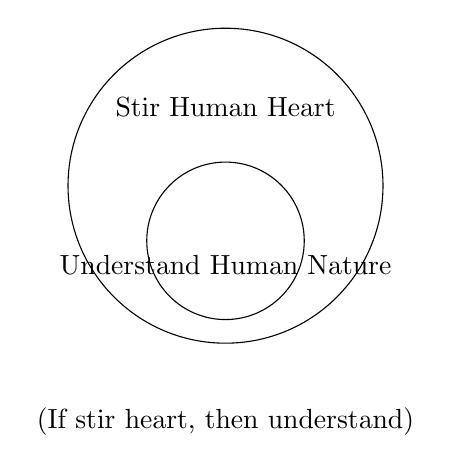
\begin{tikzpicture}
                            \draw (0,0) circle (2cm);
                            \draw (0,-0.7) circle (1cm);
                            \node at (0,-1) {Understand Human Nature};
                            \node at (0,1) {Stir Human Heart};
                            \node at (0,-3) {(If stir heart, then understand)};
                        \end{tikzpicture}
                        \end{center}
                        
                        \item For all writers \( x \), if \( x \) understands human nature, then \( x \) is clever.
                        \begin{center}
                        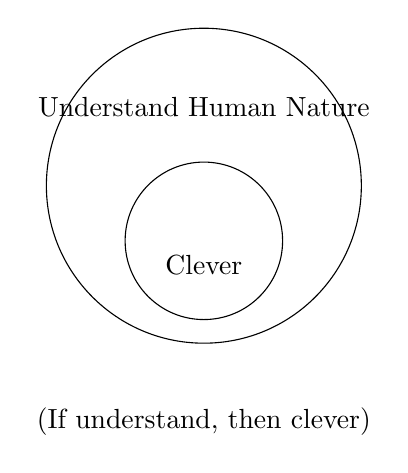
\begin{tikzpicture}
                            \draw (0,0) circle (2cm);
                            \draw (0,-0.7) circle (1cm);
                            \node at (0,-1) {Clever};
                            \node at (0,1) {Understand Human Nature};
                            \node at (0,-3) {(If understand, then clever)};
                        \end{tikzpicture}
                        \end{center}
                    \end{enumerate}
            \end{enumerate}

        \item Section 4.1 \#7, 11, 16.
            \begin{enumerate}
                \item[7.] There are real numbers $a,b$ such that 
                    \[
                    \sqrt{a+b} = \sqrt{a} + \sqrt{b}
                    \]
                \begin{proof}[proof 4.1.7]
                    let $a,b \in \R$, choose $a=0 \in \R$, $b=2 \in \R$\\
                    \[
                    \sqrt{0^2 + 2^2} = \sqrt{2^2}
                    \]
                    
                \end{proof}

                \item[11.] There is an integer $n$ such that $2n^2 5n +2$ is prime.
                    \begin{proof}[proof 4.1.11]
                        Choose $n=3 \in \Z$
                        \[
                        2\times 3^2 -5 \times 3 +2 = 5 \in \mathbb{P}
                        \]
                    \end{proof}

                \item[16.] For every integer $n$, if $n$ is even then $n^2+1$ is prime.
                    \begin{proof}[proof 4.1.16]
                        Choose $n = 8 \in \Z$
                        \[
                        8^2 + 1 = 65 \notin \mathbb{P}
                        \]
                    \end{proof}
            \end{enumerate}

        \newpage
        
        \item Section 4.1 \#22, 29.
            \begin{enumerate}
                \item[22.] For each integer $n$ with $1\leq n \leq 10$, $n^2 - n + 11$ is a prime number. 
                \begin{proof}[proof 4.1.22].\\
                    let $f(x) = x^2 - x + 11 $, \\
                    let be a statement variable whose value is $\forall n \in \Z \paren{1\leq n \leq 10}$\\
                    let $P(x)$ be the predicate $f(n) \in \mathbb{P}$\\
                    \begin{align*}
                        &n = 1\;\;\; f(n) = 11 \;\;\; P(n) \equiv \T\\
                        &n = 2\;\;\; f(n) = 13 \;\;\; P(n) \equiv \T\\
                        &n = 3\;\;\; f(n) = 17 \;\;\; P(n) \equiv \T\\
                        &n = 4\;\;\; f(n) = 23 \;\;\; P(n) \equiv \T\\
                        &n = 5\;\;\; f(n) = 31 \;\;\; P(n) \equiv \T\\
                        &n = 6\;\;\; f(n) = 41 \;\;\; P(n) \equiv \T\\
                        &n = 7\;\;\; f(n) = 53 \;\;\; P(n) \equiv \T\\
                        &n = 8\;\;\; f(n) = 67 \;\;\; P(n) \equiv \T\\
                        &n = 9\;\;\; f(n) = 83 \;\;\; P(n) \equiv \T\\
                        &n = 10\;\;\; f(n) = 101 \;\;\; P(n) \equiv \T\\
                    \end{align*}
                    $\forall n \in \Z \paren{1\leq n \leq 10}:P(n)$\\
                \end{proof}

                \item[29.]?
                
            \end{enumerate}

        \newpage
        \item Section 4.2 \#8, 9, 14.     
            \begin{enumerate}
                \item[8.] For any integer $m,n$, where $m$ is even and $n$ is odd, then $5m+3n$ is odd
                \begin{proof}:\\
                    let $m \in 2\Z$, and $n  \in \Z - 2\Z$\\
                    $m = 2k_1$ for some $k_1 \in \Z$\\
                    $n = 2k_2 + 1$ for some $k_2 \in \Z$
                    \begin{align*}
                        5m+3n &= 5\paren{2k_1} + 3\paren{2k_2 + 1} & \text{Substitution}\\
                        &= 10k_1 + 6k_2 +3\\
                        &= 2\paren{5k_1 + 3k_2 + 1} + 1\\
                    \end{align*}
                    let $5k_1 + 3k_2 + 1 = k_3 \in \Z$, since integer is closed under addition
                    \begin{align*}
                        5m+3n &= \\
                        2\paren{5k_1 + 3k_2 + 1} + 1 &= 2k_3 + 1 &\text{Substitution}\\
                    \end{align*}
                    \[
                    \therefore 5m+3n \in \Z - 2\Z
                    \]
                    
                \end{proof}
                
                \item[9.] If an integer greater than 4 is a perfect square, then the immediately preceding integer is not a prime.\\
                Re call the definition of a composite number is
                \[
                \defcomp
                \]
                    \begin{proof}[proof 4.2.8]:\\
                        let $m,n \in \Z:m>4 \wedge m = n^2$. let $k\in \Z: k = m-1$ be the preceding number.
 
                            \begin{align*}
                                &  k = n^2 - 1  & \text{Substitution}\\
                                &  k = (n-1)(n+1) & \text{Algebra}\\
                            \end{align*}
                            Where $n-1 \in \Z$ and $n+1 \in \Z$
                            Since $m\geq 4$, therefore $n > 2 \vee n < -2$.  Assume $n>2$, then
                            \begin{align*}
                                &   1 < n-1 < n < n+1 < (n-1)(n+1)\\
                                &   n-1,n+1 \in \Z^+ \\
                                &   k = (n-1)(n+1)
                            \end{align*}
                            Therefore, $k \notin \mathbb{P}$ for all perfect square $m$.
                        
                    \end{proof}


                \item[14.] There exists an integer $k\geq 4$ such that $k^2 + 2k + 1$ is prime. 
                    \begin{proof}[disproof 4.2.14]:\\
                        let $k \in \Z : k \geq 4$, let $m$ be $k^2 + 2k + 1$
                        \begin{align*}
                            &m=k^2 + 2k + 1\\
                            &m=(k+1)^2 & \text{by Algebra}\\
                        \end{align*}
                        $r,s \in \Z$ since $\Z$ is closed under addition, and $r=s=k+1$. Since $k\geq 4$, therefore
                        \[
                        1<5<k+1
                        \]
                        And
                        \[
                        1<r,\;\;\; 1<s
                        \]\[
                        1<s < rs,\;\;\; 1<r<rs
                        \]
                        And
                        \[
                        m=rs
                        \]
                        $m\in \Z$ since integer is closed under multiplication. And $m$ is a composite number.
                        
                    \end{proof}

            \end{enumerate}
        \newpage
        \item[14.] Section 4.2 \#18, 19.
            \begin{enumerate}
                \item[18.] The proof assumed the conclusion, and skipped step when demonstrating $(2p)(2q+1)=2r$.
                \item[19.] The proof assumed identical $k$ for both even integer where it should be $m=2k_1$ for some $k_1 \in \Z$ and $n = 2k_2$ for some $k_2 \in \Z$.
            \end{enumerate}

        \item[15.] Section 4.2 \#26, 30, 31
            \begin{enumerate}
                \item[26.] For integer $a,b,c$, if they are consecutive, then their sum is even.
                    \begin{proof}[disproof 4.2.26]:\\
                        Choose $a=2\in \Z$, and $b=3 \in \Z$,$c=4 \in\Z$. We have
                        \[
                        a + b + c = 9 \notin 2\Z
                        \]
                    \end{proof}

                \item[30.] For every integer $m > 2$, $m^2 - 4$ is composite. 
                    \begin{proof}[disproof 4.2.30]:\\
                        Choose $m=3>2 \in \Z$, $n = 3^2-4 = 5 \in \mathbb{P}$
                    \end{proof}

                \item[31.] For every integer $n$, $n^2 - n + 11$ is a prime number.
                    \begin{proof}[disproof. 4.2.31]:\\

                        Choose $n = 11$
                        \[
                        n^2 - n + 11 = 121 \notin \mathbb{P}
                        \]
                        
                    \end{proof}

                
            \end{enumerate}

        


        
            
    
    \end{enumerate}

    
        








\end{document}